\begin{small}
\emph{\enquote{Was haben Sie denn gegen das Lachen? Kann man denn auch
nicht lachend sehr ernsthaft sein? {[}\ldots{}{]} das Lachen erhält uns
vernünftiger als der Verdruß.}} (aus: Gotthold Ephraim Lessing (1763):
Minna von Barnhelm, 4. Akt)
\end{small}

Dieser Artikel beschäftigt sich mit Fernseh-Bildern\footnote{Zum Thema
  \enquote{die Bibliothek in der Literatur} gibt es zahlreiche
  Veröffentlichungen, hingewiesen sei an dieser Stelle auf die
  Bibliographie von Monika Bargmann, online unter:
  http://library-mistress.net/berufsbild/belletristik-film/sekundaerliteratur/Sowie
  auf die Kategorie \enquote{Bibliothek in der Literatur} im
  Libreas-Blog:
  \url{https://libreas.wordpress.com/category/sonstiges/die-bibliothek-in-der-literatur/}.

  Zum Thema \enquote{Bibliotheken im Film} sei exemplarisch auf den
  Artikel von Martin Hermann hingewiesen: Hermann, Martin (2012):
  Bibliotheksdarstellungen im Film. Ein Analysemodell und vier
  Fallbeispiele. In: Perspektive Bibliothek, 1 (2012), online verfügbar
  unter:
  \url{http://journals.ub.uni-heidelberg.de/index.php/bibliothek/article/view/9399}}
von Bibliotheken und Bibliothekaren\footnote{In diesem Artikel wird für
  die Berufsbezeichnung Bibliothekar die männliche Form gewählt.} mit
dem Schwerpunkt auf den humoristischen Genres Comedy und Komödie. Die
Leitfrage, welches vorherrschende Verständnis in ausgewählten
Fernsehsendungen dieser Genres zugrunde liegt, wird anhand einer
standardisierten, quantitativen Inhaltsanalyse analysiert. Diese
betrachtet unter anderem die Dimensionen Erscheinungsbild, Stereotypen
und Nutzungsmotive von Bibliotheken. Ebenso wird der Frage nachgegangen,
ob Bibliotheken und Bibliothekare Objekte des Witzes sind.

\subsubsection{Comedy, Komödie, Humor und das
Fernsehen}\label{comedy-komuxf6die-humor-und-das-fernsehen}

Comedy,\footnote{Der Begriff Comedy ist vielfach besetzt, im allgemeinen
  deutschen Sprachgebrauch ist für Bühnenstücke oder Fernsehfilme eher
  der Begriff Komödie gebräuchlich. Comedy wird in Zusammenhang mit
  \enquote{Stand-up-Comedy} (Bühnenshows einzelner oder mehrerer
  Künstler) verwendet.} Komödie, Humor im Allgemeinen kann man verstehen
als eine besondere Form von Kommunikation, die sich mit fast allen
Themen und Gegenständen der Gesellschaft befassen kann. Humoristisches
im Fernsehen hat in erster Linie die Funktion, die Zuschauer zu
erheitern. Komödien haben in der Regel eine dramaturgische Handlung, die
gut und glücklich für alle Protagonisten endet. Doch neben der
Unterhaltung der Zuschauer kann Humor auch kritisch sein. Humor
reflektiert Konventionen. Eine Analyse des Humors kann daher bestimmte
Strukturen gesellschaftlicher Phänomene ans Licht bringen.\footnote{Gottwald,
  Claudia (2009): Lachen über das Andere. Eine historische Analyse
  komischer Repräsentationen von Behinderung. Bielefeld :
  transcript-Verlag. \enquote{Die Analyse des Komischen als soziales,
  kulturelles oder psychologisches Phänomen ermöglicht gleichzeitig auch
  die Analyse bestimmter gesellschaftlicher Strukturen, nämlich jener,
  die im Komischen thematisiert werden.}(S. 17)} Gerade
fernsehspezifische Populärkultur wie Seifenopern, Sitcoms, Komödien
bedienen sich oft klischeehafter Rollenbilder. Ein näherer Blick auf das
Witzige mag vermuten, dass gerade dort, wo Klischees vermehrt
anzutreffen sind, eine Idee von Bibliothek und des Bibliothekar
besonders deutlich werden kann.

Die leitenden Fragen dieser Untersuchung lauten daher: Gibt es
stereotype Darstellungen von Bibliothekaren und Bibliotheken in den
humoristischen Genres und wenn ja, welche sind vorherrschend und
bestimmend? Was wird den Zuschauern in Bezug auf Bibliotheken
vermittelt? Wie werden Bibliotheken und Bibliothekare in humoristischen
Fernsehsendungen dargestellt? Welche Aufgabenzuweisung gibt es? Worüber
wird in Bezug auf Bibliotheken gelacht? Sind Bibliotheken und
Bibliothekare Objekt des Witzes?

Dies soll jedoch nicht dazu verleiten, im Medium Fernsehen die Wahrheit
im Sinne eines wahren Abbildes der Realität finden zu wollen.
\enquote{Medien können keine außermediale Wirklichkeit abbilden, sondern
nur eigene Wirklichkeiten herstellen und darstellen -- eben
Medienwirklichkeiten.}\footnote{Schmidt, Siegfried J. (2005):
  Objektivität als Medienritual. In: cover 5 (2005), S. 84} Fernsehen
schafft zudem auch eigene Realitäten, insbesondere wenn die Grenzen
zwischen Fiktion und Fakten verschwimmen. Man denke an sogenannte
\enquote{Scripted Reality Formate}, die den Zuschauern eine objektive
Dokumentation vorgaukeln, aber dennoch nach Drehbuch produziert werden
und zumeist völlig frei erfunden sind. Fernsehen als Medium ist Teil der
Lebenswirklichkeit vieler Menschen. Das Massenmedium hat Einfluss auf
Themen und Diskussionen in der Gesellschaft.\footnote{Groebel, Jo
  (2014): Das neue Fernsehen. Mediennutzung, Typologie, Verhalten.
  Wiesbaden: Springer, S. 7} Die Zuschauer nehmen dabei die Programme
als Angebot wahr, die sie unterschiedlich interpretieren, was Teil ihrer
Realität werden kann. Fernsehinhalte oder auch Formate können zum
Gesprächsstoff werden, bis hin zu Fankreisen und Subkulturen, die sich
ausprägen können.\footnote{Holly, Werner (2004): Fernsehen. Tübingen:
  Niemeyer, S. 81} Fernsehen bietet Angebote, die von Zuschauern genutzt
werden können, indem sie sich auf eine Interaktion einlassen.\footnote{vgl.
  Mikos, Lothar (2003): Film- und Fernsehanalyse. Konstanz:
  UVK-Verlags-Gesellschaft, S. 21} Doch wie die Zuschauer diese Angebote
nutzen ist sehr unterschiedlich. Keppler spricht von einem realistischen
Konstruktivismus: \enquote{Die Inszenierungen des Fernsehens erzeugen
nicht die Realität jenseits ihrer Bilder, aber sie generieren
Verständnisse, die, wenn sie intersubjektiv und öffentlich wirksam
werden, die Realität durchaus modifizieren.} \footnote{Keppler, Angela
  (2006): Mediale Gegenwart: eine Theorie des Fernsehens am Beispiel der
  Darstellung von Gewalt. Frankfurt a.M.: Suhrkamp, S. 10}

Fernsehen als Massenmedium ist gleichzeitig ein Einwegmedium,\footnote{Holly
  (2004), S. 8} die produzierten Inhalte werden von einem Produzenten
(Sender) an einen Zuschauer (Rezipienten) gesendet, der diese auf
unterschiedliche Arten empfängt oder konsumiert. Monokausale
Wirkungsannahmen, wie ein \enquote{Stimulus-Response-Modell}, dass diese
Sendungen beim Empfänger quasi automatisch eine Wirkung auslösen, sind
mittlerweile überholt.\footnote{Holly (2004), S. 76} Das Gesendete wird
nicht einfach gesehen, aufgenommen und verarbeitet. Es ist vielmehr mit
einer Rezeption \enquote{ein hohes Maß an Selektivität, an
eigenständigem Umgang mit dem Fernsehtext verbunden {[}\ldots{}{]}, was
in der Tradition der \enquote{Cultural Studies} als \enquote{Aneignung}
konzeptualisiert worden ist. Dabei ist vorausgesetzt, dass jeder Text
grundsätzlich mehrdeutig und damit offen ist, so dass unterschiedliche
Lesarten zum Tragen kommen können.}\footnote{Holly (2004), S. 78}
Kurzum, als Massenmedium spiegelt Fernsehen gesellschaftliche Themen und
ist gleichwohl Teil von Diskussionen. Das Reizvolle am Medium Fernsehen
ist für viele Menschen immer noch

\begin{quote}
\enquote{professionell gemachte, überraschende und unterhaltsame Inhalte
{[}\ldots{}{]}, die ihnen unaufwändigen Konsum ermöglichen.
{[}\ldots{}{]} Und mit rund 95 Prozent der deutschen Haushalte, die
einen Fernsehanschluss haben, liegt es immer noch fast 20 Prozent
oberhalb der Quote für einen aktiv genutzten Online-Zugang.}\footnote{Groebel
  (2014), S.9}
\end{quote}

Im Schnitt empfängt jeder deutsche Haushalt derzeit 80 Sender. Fast alle
diese Sender strahlen rund um die Uhr (etwa 8700 Stunden im Jahr) ein
Programm aus. Der Fernsehkonsum ist, trotz Internetnutzung und anderer
Medien immer noch relativ hoch. Jeder oder jede Deutsche schaut
statistisch im Schnitt etwa drei Stunden (221 Minuten) täglich
fern.\footnote{Zubayr, Camille; Gerhard, Heinz (2014): Tendenzen im
  Zuschauerverhalten. Fernsehgewohnheiten und Fernsehreichweiten im Jahr
  2014. In: Media Perspektiven. 3 (2015), S. 114. Online verfügbar
  unter:
  \url{http://www.ard-werbung.de/media-perspektiven/publikationen/fachzeitschrift/2015/heft-3/}
  (letzter Zugriff: 12.10.2015)}

\subsubsection{Methode}\label{methode}

Um eine erwartete größere Anzahl von Sendungen quantitativ auf eine
bestimmte Fragestellung und ein Erkenntnisinteresse hin zu untersuchen,
eignet sich die empirische Methode der Inhaltsanalyse. Das Material wird
anhand vorab definierter Merkmale (Kategorien) analysiert. Nachteil
dieser Methode bleibt jedoch, dass sie sich nicht mit allen
Bedeutungsebenen oder sich mit der Ästhetik einzelner Werke befassen
kann.

\begin{quote}
\enquote{Die Inhaltsanalyse ist eine empirische Methode zur
systematischen, intersubjektiv nachvollziehbaren Beschreibung
inhaltlicher und formaler Merkmale von Mitteilungen, meist mit dem Ziel
einer darauf gestützten interpretativen Inferenz auf mittelungsexterne
Sachverhalte.}\footnote{Früh, Werner (2015): Inhaltsanalyse. Theorie und
  Praxis. 8., überarb. Aufl. Konstanz: UVK Verlagsges., S. 29}
\end{quote}

Dabei wird bei der Kategorienbildung sowohl theoriegeleitet (aus den
Forschungsfragen sowie aus Erkenntnissen, die gegebenenfalls aus anderen
Untersuchungen vorliegen) als auch empiriegeleitet (aus dem Material
selbst, ersten Stichprobenanalysen) vorgegangen. Aus einem angenommenen
Stereotyp \enquote{Brille, Dutt, zurückhaltend, grau} ergeben sich die
zu untersuchenden Dimensionen Erscheinungsbild und
Charaktereigenschaften für die Figur von Bibliothekaren. Als Klischee
der Bibliothek \enquote{verstaubt, unmodern} wären die Dimensionen
Darstellung, Atmosphäre, sowie Nutzungsmotive von Interesse. Bei einigen
Aspekten wird dabei mit offenen Kategorien gearbeitet, zum Beispiel bei
der Frage \enquote{worin besteht der Witz}? Zudem wurden konkrete
Aussagen oder Off-Kommentare transkribiert und diese in der Analyse
nachträglich nach Kategorien geclustert, um Aspekte erfassen zu können,
die im Vorfeld nicht bedacht werden konnten.

Das relevante Quellenmaterial wurde über eine bewusste Auswahl anhand
einer Recherche in Online-TV-Zeitschriften zusammengestellt. Über einen
längeren Zeitraum von 5 1/2 Jahren wurden über eine inhaltliche Suche
nach den Begriffen \enquote{Bibliothek*} und entsprechender Synonyme in
den Sendungsinhalten, Hintergrundinformationen oder Rollenbeschreibungen
relevante Sendungen ermittelt. Ein Sampling-Verfahren der sogenannten
künstlichen Woche, in welcher Sendungen verschiedener Wochentage über
einen bestimmten Zeitraum ausgewählt werden, so dass jeder Wochentag in
gleicher Anzahl vorkommt, oder eine Stichprobenziehung bei der
Gesamteinheit aller Komödien und Comedysendungen, die ausgestrahlt
werden, wäre noch zeitaufwändiger gewesen, um an relevantes
Quellenmaterial zu gelangen und daher nicht umgesetzt. Die
Auswahleinheiten wurden zudem nur von frei zu empfangenden
Fernsehsendern bezogen, Pay-TV und reine Lokalsender wurden
ausgeschlossen, ebenso ausländische Sender, auch, wenn diese ein
deutschsprachiges Programm anbieten. Aufgrund der Flüchtigkeit des
Mediums Fernsehen war es notwendig, alle Sendungen aufzuzeichnen. Der
Vorteil liegt jedoch darin, dass das Material für eine Analyse dauerhaft
vorliegt. Der betrachtete Zeitraum bezog sich auf Januar 2010 bis Juli
2015.

Aus diesen Auswahleinheiten wurden dann die tatsächlichen
Analyseeinheiten selektiert. Nur Sendungen, in welchen tatsächlich eine
Handlung in einer Bibliothek stattfindet und / oder eine Rolle als
Bibliothekar vorkommt und die den Genres Komödie, Comedy, Sitcom
zuzuordnen sind, wurden analysiert. Als Definition des
Untersuchungsgegenstandes wurden alle Fernsehsendungen betrachtet, die
beabsichtigen, beim Zuschauer unterhaltend zu wirken, insbesondere
fiktionale Formate mit dem Schwerpunkt auf Humor für die Zielgruppe
Jugendliche bis Erwachsene. Kindersendungen und andere Formate mit teils
humoristischen Elementen wurden ausgeschlossen.

Als Analyseeinheiten wurden in dem gewählten Zeitraum insgesamt 51
einzelne Sendungen identifiziert. Wiederholungen wurden nicht erfasst.
Aus den Sendedaten erkennbar war jedoch, dass insbesondere aktuellere
Produktionen eine auffällig hohe Wiederholungsfrequenz haben. Eine
Stichprobe bei den zwei aktuellsten Sendungen ergaben sich
Wiederholungsraten von 18 beziehungsweise 30 Mal seit der
Erstausstrahlung bezogen auf einen Sender.\footnote{Die Folge
  \enquote{die Menschenflüsterin} aus der Sitcom \enquote{Two and a half
  men} lief seit der Erstausstrahlung im Februar 2013 auf Pro7 dort 18
  Mal bis Mitte Juli 2015. Die Folge \enquote{Prinzessinnen der
  Wissenschaft} aus der Sitcom \enquote{Big Bang Theory} lief 30 mal
  seit Erstausstrahlung vor zwei Jahren auf Pro7 bis Juli 2015.} Diese
Stichprobenergebnisse der zahlreichen kurzfristigen Wiederholungen wird
gestützt durch den Blick in die aktuelle Programmanalyse der deutschen
Hauptsender (RTL, RTLII, vox, Sat1, Pro7, Kabel1, ARD, ZDF). Über 25
Prozent des Programms (sechs bis sieben Stunden pro Tag) privater Sender
besteht aus sogenannten kurzfristigen Wiederholungen, bei den
öffentlich-rechtlichen Sendern (ARD/ZDF) sind es deutlich weniger mit
drei bis vier Stunden pro Tag.\footnote{Programmbericht 2014 (2015).
  Fernsehen in Deutschland. Programmforschung und Programmdiskurs.
  Hrsg.: die Medienanstalten, ALM GbR. Leipzig: vistas, S. 49 Online
  verfügbar unter:
  \url{http://www.die-medienanstalten.de/publikationen/programmbericht.html}
  (letzter Zugriff: 10.10.2015)}

\subsubsection{Formale Ergebnisse}\label{formale-ergebnisse}

Die Analyse ergab, dass allein 42 der 51 Sendungen von Privatsendern
ausgestrahlt wurden. Dieser hohe Anteil liegt nicht darin begründet,
dass öffentlich-rechtliche Sender weniger Unterhaltungssendungen zeigen
würden, sondern an einem relativ hohen Anteil an Fremdproduktionen bei
den Privatsendern, wie weiter unten näher erläutert wird.

ARD und ZDF liegen mit ihrem Anteil an Informationssendungen zwar
deutlich vor den Privatsendern, der Anteil fiktionaler Sendungen des
Programms liegt jedoch bei den öffentlich-rechtlichen Sendern direkt an
zweiter Stelle. Die aktuellen Programmanalysen zeigen,\footnote{Die
  Programmstruktur der fünf größten deutschen Sender (ARD, ZDF, RTL,
  Sat1, Pro7) wird regelmäßig analysiert. S. Krüger, Udo Michael (2015):
  Profile deutscher Fernsehprogramme. Tendenzen in der
  Angebotsentwicklung. In: Media Perspektiven. 3 (2015), S. S. 146} dass
ARD und ZDF mit 36 \% beziehungsweise 32 \% sogar mehr fiktionale
Sendungen ausstrahlen als RTL (rund 20 \%) und Sat1 (rund 28 \%). Pro7
sticht allerdings mit einem hohen Fiktionsanteil von 61 \% heraus. Pro7
hat bei den ermittelten 51 Sendungen einen Anteil von 9 \%, wobei eine
weitere Interpretation hier zur Verzerrung führen würde, da die
Sendungen auch in ihren Wiederholungen von unterschiedlichen Sendern
gezeigt werden.

\begin{quote}
\enquote{Das größte Gewicht unter den Fictionformen hatten weiterhin bei
allen Sendern die Fernsehserien. Dabei behauptete sich ProSieben (46,9
\%) mit nochmals gestiegenem Angebot und wachsendem Abstand zu den
übrigen Sendern wieder als größter Serienanbieter. Unter den vier
anderen Sendern rangierte das ZDF (20,5 \%) vor der ARD (18,2 \%),
gefolgt von Sat.1 (16,2 \%) und RTL (13,7 \%).}\footnote{Krüger (2015),
  S. 153}
\end{quote}

Nur zwölf der 51 Sendungen wurden in Deutschland produziert, der
überwiegende Teil stammt aus US-Produktionen. Schaut man genauer auf die
allgemeinen Programmanalysen der Sender und dort insbesondere auf die
Verteilung von Eigen- und Fremdproduktionen, fällt auf, dass bei den
Privatsendern die Anzahl an eingekauften Fremdproduktionen relativ hoch
ist, insbesondere bei Fernsehserien und Sitcoms. ARD und ZDF liegen mit
zehn beziehungsweise 13 Prozent bei einem relativ geringen Anteil von
US-Importen. RTL (51 \%), Sat.1 (79 \%) und vor allem Pro7 (93 \%)
bestreiten ihr Fiktionsprogramm zum Großteil aus US-Importen.\footnote{vgl.
  Krüger (2015), S. 161/162} Dies lässt den Rückschluss zu, dass das
Bild der Bibliotheken und Bibliothekare in den Genres Comedy und Komödie
vor allem ein US-amerikanisch geprägtes Bild ist.

Bei den analysierten 36 Sendungen handelt es sich um einzelne Folgen aus
Serien, daneben wurden 15 Filmkomödien mit Bibliotheksbezug
ausgestrahlt. Die knapp 50 verschiedenen Sendungen lassen sich auf
verschiedene Sub-Genres aufteilen (Sitcoms (19), Comedyserien (3),
Sketchshows (8), Zeichentrickserien (5), Filmkomödien (16)). Zunächst
sind die Sitcoms zu nennen. Sitcoms sind Comedyserien mit festen
Rollencharakteren, bei welchen der Humor aus Alltagssituationen
(Situationskomödie) generiert wird, \enquote{die geprägt sind von
Missverständnissen, Konfusionen, Verwechslungen, Stereotypen.}\footnote{Faulstich,
  Werner (2008): Grundkurs Fernsehanalyse. Paderborn: Fink, S. 58}
Entstanden sind die Sitcoms in den USA. \enquote{Die gesamte
Inszenierung ist theaternah, was durch die Einblendung von fingierten
Publikumsreaktionen (}canned audience\enquote{) noch verstärkt
wird.}\footnote{Holly (2004), S. 65} Um sie von deutschen Sendungen zu
unterscheiden, die in ihrer Produktion und Ausstattung abweichen, ist
bei deutschen Sendern der Begriff Comedyserie üblich. Davon finden sich
unter den 51 Analyseeinheiten nur zwei Sendungen (\enquote{Nikola},
\enquote{Mein Leben und ich}), sowie eine in Großbritannien produzierte
Serie (\enquote{Suburban shootout}).

Neben den Sitcoms und Comedyserien findet sich ein weiteres
humoristisches Subgenre mit der Sketchshow. Als Sketchshow gelten eher
\enquote{gespielte Witze} in lockerer Aneinanderreihung. Es kann auch
hier wiederkehrende Rollencharaktere geben (beispielsweise Little
Britain), aber eine durchgehende Handlung ist nicht üblich. Als weiteres
Subgenre können satirisch-komische Zeichentrickserien gelten. Bei fünf
Sendungen handelt es sich um Folgen der \enquote{Simpsons}, eine
Zeichentrickserie, die auf satirisch-komische Art das Alltagsleben der
US-Gesellschaft darstellt. Bei den 16 Filmkomödien, darunter auch eine
Zeichentrickkomödie, ergeben sich jeweils abgeschlossene dramaturgische
Handlungen, die glücklich enden. Eine unterhaltende Grundstimmung soll
oft durch Missverständnisse, die sich im Nachhinein auflösen, oder
übertriebene Darstellungen menschlicher Schwächen entstehen.

Kabarett als humoristisches Subgenre wurden nicht gefunden. Zum einen
kann es daran liegen, dass fiktionale Figuren in diesem Genre seltener
anzutreffen sind oder das Motiv Bibliothek weniger attraktiv für
Kabarettisten ist. Vermutlich ist die Erschließung durch
Online-Zeitschriften nicht ausreichend. Zumindest ein Fall einer Figur
im Kabarett ist bekannt.\footnote{\enquote{Quo vadis Mensch? : In
  \enquote{Der kaltwütige Herr Schüttlöffel} spielt Kabarettist Thomas
  Freitag einen Bibliothekar und beklagt sich über zunehmenden
  Kulturverfall}, In: BuB Jg. 67, 1 (2015), S. 69}

Die Produktionsjahre der 51 Sendungen weisen eine erhebliche Streuung
auf. 47 Sendungen wurden vor dem betrachteten Zeitraum 2010-2015
produziert.\footnote{37 Sendungen wurden vor 2005 produziert und sind
  damit älter als Libreas :-)} , davon wurden 37 Sendungen bereits vor
2005 produziert. Bei den ältesten zwei Sendungen handelt es sich um zwei
deutsche Spielfilme aus den Jahren 1956 und 1957. Vierzehn Sendungen
wurden in den 1980er und 1990er produziert und ab 2000 wurden 19
Sendungen gedreht. Ein Peak liegt auf dem Produktionsjahr 2003, hier
liefen gleich zehn einzelne Folgen mit Bibliotheksbezug in den
Sketchshows \enquote{Die dreisten Drei} und \enquote{Little Britain}.
Daraus lässt sich schließen, dass die Comedy- und Komödiensendungen mit
Bibliotheksbezug vor allem aus sogenannten Konserven bestehen
(Wiederholungen). Wie bereits erwähnt werden dabei die aktuelleren
Sendungen deutlich häufiger wiederholt als die älteren.

\subsubsection{Die Figur des
Bibliothekars}\label{die-figur-des-bibliothekars}

In 32 Sendungen findet sich die Figur der Bibliothekarin beziehungsweise
des Bibliothekars. Dabei treten in sieben Sendungen gleich zwei Figuren
auf, so dass es insgesamt 39 Figuren gibt, die für die Analyse relevant
sind. Bibliothekare , die nicht am Arbeitsort Bibliothek gezeigt wurden,
gibt es in fünf Sendungen. In den überwiegenden Fällen handelt es sich
um kurze Szenen, in welchen Bibliothekare eine Rolle spielen. In fünf
Filmen ist die Figur gleichzeitig Protagonist.

Für alle Figuren wurde ein wertender Gesamteindruck betrachtet. Dabei
lag eine einfache Skala mit mittlerer Ausprägung zugrunde
(positiv/neutral/negativ), sowie eine Auffangkategorie bei nicht
wertbaren Szenen, wenn zum, Beispiel die Rolle zu kurz gestaltet war
(Statisten). Die Kriterien wurden vorab im Rahmen der Inhaltsanalyse
festgelegt, beschrieben und anhand von mindestens einem Ankerbeispiel
erläutert.

Die meisten Figuren werden positiv dargestellt, überwiegend freundlich,
hilfsbereit, lächelnd und den anderen Figuren entgegenkommend. Sieben
Figuren sind negativ dargestellt, hier gibt es unterschiedliche
Charaktereigenschaften wie sehr streng und zurückweisend, oder chaotisch
und verwirrt oder sehr introvertiert und nicht entgegenkommend. Bei neun
Figuren sind sowohl positive als auch negative Kriterien
Charaktereigenschaften feststellbar, oder die Figuren sind nicht so
deutlich ausgestaltet, so dass sie als neutral gewertet wurden. Bei fünf
Sendungen sind die Szenen so kurz, dass sie nicht bewertet werden
können. Ein geschlechtsspezifischer Unterschied in der Gesamtbewertung
nach Charaktereigenschaften lässt sich nicht feststellen.

Das Erscheinungsbild der Bibliothekar-Figuren weist in den überwiegenden
Fällen einen konservativeren Kleidungsstil auf. In Relation zu den
anderen Figuren ist der Kleidungsstil eher konservativ oder
zurückhaltend, hochgeschlossen, mit gedeckten Farben. Ein Dutt bei
Frauen ist bis auf zwei Sendungen nicht anzutreffen. Ein Stereotyp einer
strengen Bibliothekarin mit Dutt und Brille, die mit einem \enquote{Shh}
zur Ruhe mahnt, war gar nur in einem Fall der 51 Sendungen anzutreffen.
Bei den weiblichen Figuren ist auffallend, dass hier eine Tendenz in den
aktuelleren Produktionen erkennbar ist, in welchen die Figuren weniger
hochgeschlossen und mit kräftigeren Farben gekleidet waren. Man könnte
diese Figuren mit dem Attribut \enquote{attraktiver} belegen. Auffällig
ist hier, dass es sich um Rollen handelt, die im Rahmen der
dramaturgischen Handlung in einer Beziehungsebene mit anderen Figuren
stehen. Vermutet werden kann, dass sich das
\enquote{Geschlechterstereotyp Frau} als attraktive Partnerin
überlagert. Bei den männlichen Figuren ist im Vergleich zu den anderen
Figuren der untersuchten Serien der konservative, zurückhaltende
Kleidungsstil zu beobachten: hochgeschlossen, Hemd, Krawatte, Pullunder
oder Anzug und Weste. Eine Tendenz zum legeren Kleidungsstil ist nicht
festzustellen, allerdings taucht nach dem Produktionsjahr 2006 keine
männliche Figur mehr in den Sendungen auf.

%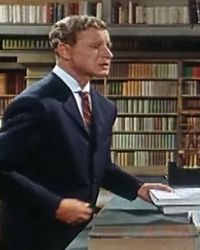
\includegraphics{img/wennwir.jpg} 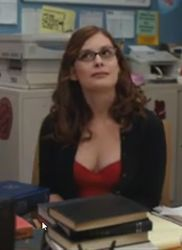
\includegraphics{img/Community.jpg}

Ein zeitlicher Wandel ist im Vergleich der Produktionen durchaus
erkennbar. Am deutlichsten fällt dies beim Vergleich auf, vergleicht man
die der Figuren aus der ältesten Sendung aus 1956 (\enquote{Wenn wir
alle Engel wären}) mit der jüngsten Sendung aus 2011
(\enquote{Community, Folge Liverpool gegen Manchester}) auf. 1956
treffen wir auf die Form der Thekenbücherei, hier sucht der Bibliothekar
die Lektüre für seine Leser aus. Sein Leitspruch ist \enquote{Ordnung,
Sauberkeit und Pflichtbewusstsein}.

Im Vergleich zu den anderen Figuren ist das äußere Erscheinungsbild
konservativer und die anfangs dargestellte Charaktereigenschaft auch
eher mit \enquote{steif} zu beschreiben. 2011 treffen wir auf eine
Bibliothek, die räumlich nicht genau zu erfassen ist. Es gibt einen
zentralen multifunktionalen Gruppenarbeitsraum mit Multifunktionalität.
Die Tätigkeiten der Figur der Bibliothekarin werden zwar durch ein
\enquote{Bücherordnen} dargestellt, sie empfiehlt jedoch nichts, selbst
gegen von Nutzern mitgebrachtes Essen hat die Figur nichts einzuwenden.
Diese Figur ist deutlich moderner und fällt im Vergleich zu den anderen
Figuren der Sendung nicht als \enquote{anti-konform} auf. Dennoch wird
sie durch die anderen Figuren mit den Funktionen \enquote{Wissen
bewahren} und \enquote{Ordnung herstellen} beschrieben: \enquote{Sie
hütet das Wissen. Sie hat die Antwort auf all' unsere Fragen} -
\enquote{Vielleicht schimpft sie mit uns, wenn wir laut sind?}

Eine Besonderheit stellen die Bibliotheksfiguren dar, die in
Filmkomödien gleichzeitig Protagonisten sind. Häufig typisch für die
Dramaturgie eines Films ist der klassische Dreiakte aus
Theaterinszenierungen mit den Bestandteilen Exposition, Konflikt und
Lösung des Konflikts (in Komödien in komischer Weise)-.\footnote{Vgl.
  Koebner, Thomas (Hrsg.) (2007): Reclams Sachlexikon des Films, 2.
  aktualisierte und erw. Aufl. Stuttgart: Philipp Reclam jun., S. 158}
\enquote{Jede erfahrene Dramaturgie wird dafür plädieren, dass die
Hauptfiguren eine Art Wandlung durchlaufen, so dass sie am Ende nicht
mehr dieselben sind wie zu Beginn.}\footnote{Koebner (2007), S. 160} In
den fünf Filmen, in welchen die Protagonisten gleichzeitig Bibliothekare
sind, wird in der Exposition eine Eigenschaft als Bibliothekar deutlich
herausgestellt, wobei dies in den Sendungen unterschiedliche
Eigenschaften sind. Der Protagonist vollzieht beispielsweise im Film
\enquote{Wenn wir alle Engel wären} eine Wandlung vom strengen, auf
Ordnung bedachten \enquote{Herrn Stadtbibliothekar} zum eher
gelasseneren Mann, der gelernt hat, dass niemand perfekt ist und man
auch mal Fehler machen kann. Ein weiteres Beispiel findet sich im Film
\enquote{Idiocracy}, in welcher welchem der Bibliothekar anfangs als
faul und verantwortungsscheu dargestellt wird (Off-Kommentar:
\enquote{Er ist der durchschnittlichste Durchschnittsmensch.}). Am Ende
der Handlung ist er zum mutigen und verantwortungsvollen Mann geworden,
der schließlich Präsident wird.

\subsubsection{Darstellung von
Bibliotheken}\label{darstellung-von-bibliotheken}

In den untersuchten Sendungen werden unterschiedliche Bibliothekstypen
sichtbar. Die häufigste anzutreffende Form ist die Öffentliche
Bibliothek. In den deutschen Produktionen tauchen Öffentliche
Bibliotheken kaum auf oder es ist nicht erkennbar, um welchen Typus es
sich handelt, wie in elf weiteren Fällen, in denen der Typus nicht
erwähnt wird oder auch keine Einstellung des Gebäudes von außen gezeigt
wird. In 16 Fällen handelt es sich um Universitäts-, College- oder
Highschool-Bibliotheken. Da die Sendungen überwiegend in den USA
produziert wurden (33 Sendungen US-Importe), handelt es sich auch um
amerikanische Bibliothekstypen.

In den USA gibt es nicht nur eine höhere Bibliotheksdichte, Bibliotheken
sind in der US-Gesellschaft auch fester verankert als in
Deutschland,\footnote{Bibliothek 2007 -- Internationale
  Best-Practice-Recherche (2004). Hrsg.: Bertelsmann Stiftung,
  Bundesvereinigung Deutscher Bibliotheksverbände e.V. Gütersloh:
  Bertelsmann Stiftung, S. 7} und sie zeichnen sich deutlicher durch
Bürgernähe und Service aus. \footnote{US-Bibliotheken verstehen sich als
  Teil der Gesellschaft, \enquote{sie sind Teil des sozialen Umfelds.
  Angebot und Image sind von Einwohnern der Kommune geprägt.} Courzakis,
  Irini (2006): Der American way of Library : US-Bibliotheken als
  Treffpunkt, Servicecenter und Bildungsstätte, In: BuB 58 (2006) 11/12,
  S. 760} Bürger der USA zählen ihre Bibliotheken mit einer hohen
Selbstverständlichkeit zu einem Teil ihres Lebens.\footnote{Simon,
  Elisabeth (1988): Bibliothekswesen in den USA. München: Saur, S. 31}
Auch kommt den Schulbibliotheken eine wichtige Rolle zu.\footnote{Bibliothek
  2007 -- Internationale Best-Practice-Recherche (2004), S. 48} Daher
ist es auch nicht verwunderlich, dass Bibliotheken in den
Medienrealitäten der US-Produktionen häufig vorkommen. Dem Umstand, dass
deutsche Privatsender einen hohen Anteil an US-Produktionen senden,
\enquote{verdanken} wir es, dass die Bibliotheken im Fernsehen häufiger
zu sehen sind.

Die Darstellung der Bibliotheken ist insbesondere in den
US-amerikanischen Sitcoms durch wiederkehrende Ausstattungsmerkmale
anzutreffen. Regalreihen an den Wänden, zumeist dunkle Holzregale und
mittig im Raum stehende Tische und Stühle als Lesebereich werden
überwiegend als Hintergrund gezeigt.

%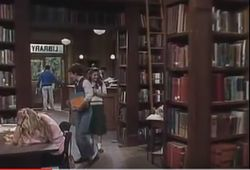
\includegraphics{img/image28.jpeg} 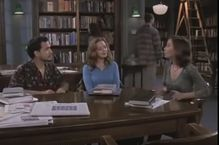
\includegraphics{img/image29.jpeg}
%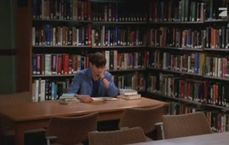
\includegraphics{img/image30.jpeg}

Man könnte meinen, die Produktion aus 2012 hätte dieselbe Ausstattung
aus 1987 verwenden können. Diese typisch für Sitcoms verwendete Szenerie
liegt darin begründet, dass die Handlungen, die überwiegend
sprachbasiert sind und durch Dialoge vorangetrieben werden, auch für den
Zuschauer deutlich im Bild sein müssen. Die Bibliothek als Raum wird zu
Beginn einer Szene oft in einer Totalen (Kameraeinstellung) dargestellt,
damit der Zuschauer sich orientieren kann. Dann wird sich in einer
Halbnah-Einstellung (Hüfte-Kopf) wieder den Figuren und ihren Dialogen
zugewendet. Die Ausstattung gleicht einer Kulisse aus dem Theater, was
wiederum typisch für Sitcoms ist, die sich aus Theaterkomödien
entwickelt haben, überwiegend in Studios als an realen Orten gedreht
werden und daher auch nur wenige Schauplätze (\enquote{Settings})
aufweisen. Die Atmosphäre in der Bühnenausstattung der Sitcoms ist eher
dunkel (es gibt in Sitcoms auch keine Fenster), aber nicht verstaubt
oder muffig, sondern überwiegend einladend und gemütlich. Dies trifft
auf die überwiegende Zahl der anderen Sendeformate ebenfalls zu. Auf die
aktuell im Bibliotheksbereich diskutierte Aufenthaltsqualität und den
Wohlfühlort nimmt man in den produzierten Sendungen keine Rücksicht. Es
gibt keine Sofas, keine Lounge und überhaupt wenig Variationen in der
Ausstattung. Die Vermutung liegt nahe, dass der TV-Zuschauer sonst
Schwierigkeiten hätte, die Szenerie als Bibliothek zu erkennen. Um eine
Szene für Zuschauer eindeutig werden zu lassen, gilt als ein Kriterium
für den Arbeitsprozess von Drehbuchautoren zum Beispiel die Frage
\enquote{Wird das Publikum diese Ausstattung, die es erst einmal und
dazu nachts gesehen hat, wiedererkennen?}\footnote{Koebner (2007), S.
  160} Ist also eine Bibliothek ohne eine \enquote{Büchertapetenkulisse}
nicht als solche erkennbar?

Ein Computer in diesen 51 Sendungen taucht zum ersten Mal in einer
europäischen Spielfilm-Produktion von 2002 auf (\enquote{Der Typ vom
Grab nebenan}, Schweden). Dies bleibt ein äußerst seltenes Bild. Für den
Ort Bibliothek in humoristischen Fernsehgenres sind eindeutig Bücher das
konstitutive Merkmal. In Spielfilmen ist die dargestellte Ausstattung
durchaus vielfältiger, wenn längere Szenen in realen Bibliotheken
gedreht wurden. Hierbei werden variationsreichere Einstellungen gezeigt
(Personen zwischen den Regalen, vor Katalogen, beim Lesen), wenngleich
das Bücherregal auch hier vorherrschendes Ausstattungsmerkmal ist. Die
Atmosphäre wirkt heller als in den Sitcoms. Das Szenenbild in der Sitcom
\enquote{Community}(2011) weicht allerdings deutlich von anderen
Produktionen ab. Hier treten die Regale in den Hintergrund, zu sehen
sind nur noch kleinere Bücherwagen in einem Multifunktionsraum, der als
Gruppenarbeitsraum mit Scanner, Flipchart und Tafel ausgestattet ist.

Drehbuchautoren bedienen sich oft vorgegebenen genrespezifischen
Mustern, wie zum Beispiel einer Schießerei in einem Western oder einer
Verfolgungsjagd in einem Actionfilm. Zudem bedingen auch typische
Standardsituationen ihrerseits typische Handlungsabläufe und
Ablaufschemata in einer Dramaturgie, wie etwa Begrüßungs- oder
Abschiedsrituale, ein Essen, ein Streit oder die \enquote{Rettung in
letzter Sekunde}.\footnote{Vgl. Koebner (2007), S. 156/S. 157}

\begin{quote}
\enquote{Der dramaturgische Vorteil der Verwendung von
Standardsituationen liegt auf der Hand. Das Publikum erkennt die
Situation wieder und kann kennerhaft auf die spezifische Nuance
reagieren. Vordem schon hat das Team, das den Film dreht (Regie, Kamera,
Schauspieler und so weiter), die Chance erkannt, ein Stereotyp in je
eigener Weise zu modellieren und damit auch die abstrakte Formel zu
verbergen, die sich für die Analyse hinter jeder Standardsituation
verbirgt.}\footnote{Koebner (2007), S. 157}
\end{quote}

Spezifische Handlungsabläufe können auch an bestimmten Orten
stattfinden, wie in einem Restaurant, in einem Altersheim oder in einer
Bibliothek. Diese Orte bestimmen zwar nicht den typischen Ablauf, aber
sie werden mit ihren Spezifika Teil der typischen Standardsituation.
Bestimmte Verhaltensregeln sind für einen bestimmten Ort konstitutiv und
kennzeichnend.\footnote{Koebner (2007), S. 160} Für eine
Bibliotheksszene bedeutet dies, dass die Bibliothek als Schauplatz mit
ihren eigenen Charakteristika, die die Drehbuchautoren als solche
bestimmen, diese Standardsituationen mitformen. Für eine
\enquote{Begrüßung} oder ein \enquote{Kennlernen} bedeutet dies zum
Beispiel, dass man zwischen Regalen steht oder sich leise unterhält,
oder von anderen Figuren zur Ruhe ermahnt wird. Humoristische Subgenres
erlauben als Drehbuchautor oder Produzent eine kreativere Umgangsweise
mit diesen Charakteristika.

\subsubsection{Witz und Bibliothek}\label{witz-und-bibliothek}

Vorherrschendes Paradigma in der Humorforschung ist der Ansatz der
Inkongruenz-Theorie. Humor ist oft dadurch bedingt, dass Situationen
oder Themen in unterschiedlichen oder gegensätzlichen
Wahrnehmungsbezügen betrachtet werden.\footnote{Räwel, Jörg (2005):
  Humor als Kommunikationsmedium. Konstanz: UVK Verl.ges., S. 15}

\begin{quote}
\enquote{Nicht jede Inkongruenz verursacht Lachen, aber die ist
wahrscheinlicher je stärker von einer spezifischen Erwartung abgewichen
wird {[}\ldots{}{]} dies {[}gilt{]} nur in Fällen {[}\ldots{}{]}, in
denen der Überraschungseffekt als nicht bedrohlich empfunden wird. Der
Humor {[}\ldots{}{]} wird vielmehr so präsentiert, dass
charakteristische Hinweise gegeben werden, dass die Situation nicht
ernst zu nehmen ist.}\footnote{Räwel (2005), S. 16}
\end{quote}

In einer Szene in der Sketchshow \enquote{Die Dreisten Drei} liegt das
Humoristische darin, dass man als Zuschauer in einer Bibliothek im
Allgemeinen Ruhe erwartet, was auch für das Verhalten des Personals
gilt, das in Bibliotheken arbeitet. Der Zuschauer sieht und hört jedoch
einen Bibliotheksmitarbeiter bei einer Führung durch ein Megafon rufen
\enquote{bitte absolute Ruhe}, wobei der Mitarbeiter derjenige ist, der
die Ruhe stört. Solche Durchbrechungen von Erwartungen finden sich in
Sketchshows häufiger als in Sitcoms oder Filmkomödien. In letzteren
Genres basiert der Humor eher auf unterschiedlichen Alltagssituationen
(Situationskomik) oder der Schaffung und Auflösung von
Missverständnissen. Liegt der Humor an der Grenze des sogenannten
\enquote{schwarzen Humors} oder der Satire, die in unterhaltsamer Form
auch eher auf eine Kritik zielt, liegt es oft im Auge des Betrachters,
ob eine Szene humorvoll gesehen wird. In einer Folge der englischen
Sketchshow \enquote{Little Britain} beispielsweise, kümmern sich zwei
Therapeuten um die Figur Anne. Anne ist ein Mann, der in Frauenkleidung
auftritt und dem ersten Anschein nach eine geistige Behinderung hat.
Durch verschiedene Maßnahmen soll Anne therapiert werden, was jedoch nie
Erfolg hat. In einem Sketch ist die Rolle der Anne eine Aushilfskraft in
einer Bibliothek. Anne beißt ein Buch, um es auszuleihen und stempelt
den Menschen. Die Figur bricht jedoch für einen kurzen Moment aus ihrer
Rolle aus und spricht und agiert \enquote{normal} während eines
Telefonates und stellt damit die Figuren der Therapeuten bloß. Man weiß
als Zuschauer nicht genau, wie man es einsortieren soll, es wird hier
zur Frage des individuellen Humors.\footnote{als \enquote{{[}\ldots{}{]}
  Mittel der Kritik am Paternalismus wird Behinderung heute als komisch
  inszeniert. {[}\ldots{}{]} In der mitteleuropäischen und der
  amerikanischen Gesellschaft stellt die komische Darstellung von
  Behinderung jedenfalls kein Tabu mehr dar.} Aus: Gottwald, Claudia
  (2009): Lachen über das Andere. Eine historische Analyse komischer
  Repräsentation von Behinderung. Bielefeld: transcript-Verl., S. 296}

In die Form der Satire reihen sich ebenso die Folgen der
\enquote{Simpsons} ein, wenn zum Beispiel die Bibliothekarin in einer
Bibliothek ohne Bücher sagt: \enquote{Bücher? Die sind was für Spießer
-- die Bibliothek ist ein Multimedialernzentrum für Kinder allen Alters
-- und für Penner.} In keiner der 51 Sendungen ist jedoch die Figur des
Bibliothekars Objekt des Witzes. Der Humor wird wie oben beschrieben
eher aus den Alltagssituationen heraus, im Zusammenspiel mit den
Bibliothekar-Figuren generiert, oder es liegt in den inkongruenten
Handlungen und Situationen begründet.

\subsubsection{Nutzungsmotive}\label{nutzungsmotive}

In den meisten Fällen, in denen Menschen Bibliotheken aufsuchen, tun sie
dies, weil sie dort lernen oder lesen möchten. Die Ausleihe oder
Rückgabe von Büchern steht dabei an zweiter Stelle. Die Rückgabe von
Medien ist oft mit einer Gebührenüberziehung verbunden. Mit
Überziehungsgebühren und drohenden Strafen wird insbesondere in älteren
Produktionen gescherzt. Beispielsweise gibt es in der Sendung
\enquote{Seinfeld} dazu eine spezielle Figur des Gebühreneintreibers,
einen sogenannten \enquote{Library Cop}.

Die Bibliotheken gelten in den Sendungen auch als Wissensort, hier
recherchiert man nach Informationen. Ein wichtigeres Motiv ist jedoch
die Bibliothek als Kommunikationsort. Dies liegt natürlich zum Einen im
Genre Komödie und insbesondere Sitcom verankert. Da dies
dialogorientierte Formen sind, in denen viel kommuniziert wird, bildet
die Bibliothek als Szenerie dabei keine Ausnahme. Vielfach lernen die
Protagonisten in der Bibliothek andere Figuren kennen, in vier Fällen
ist die Bibliothek auch der Ort eines \enquote{Dates} (US-Produktionen).
Eine weitere Funktionszuschreibung liegt bei der Darstellung der
Bibliothek als Rückzugsort. In vier Fällen wird die Bibliothek von den
Protagonisten oder anderen Figuren bewusst aufgesucht, um Ruhe zu
finden. Die Funktion des \enquote{Ruhebewahrers} wird in den 51
Sendungen dabei häufiger bei Nutzer-Figuren festgestellt als bei
Bibliothekar-Figuren. Der Aspekt Ruhe ist dabei eine Situation, mit der
gespielt wird (Beispiel: die oben erwähnte Sketchshow mit Megafon).

Dass die Bibliotheken Orte des Wissens und der Ruhe sind, kann man auch
durch zahlreiche Aussagen der Nutzerfiguren stützen:

\begin{itemize}
\item
  \enquote{Das ist das Fort Knox der Bücher.} (aus: \enquote{Eine starke
  Familie},

  \begin{enumerate}
  \def\labelenumi{\arabic{enumi})}
  \setcounter{enumi}{1993}
  \item
  \end{enumerate}
\item
  \enquote{Ich hab` im Internet nichts gefunden, deshalb probieren wir
  es auf die alte Art und Weise.} (aus: \enquote{Beethoven auf
  Schatzsuche}, 2003)
\item
  \enquote{Die Bibliothek ist der Schlüssel für eine gute Ausbildung.}
  (aus: \enquote{Hör mal wer da hämmert}, 1994)
\item
  \enquote{Hier halte ich mich am liebsten auf.} (aus: \enquote{Gilmore
  Girls}, 2004)
\item
  \enquote{Ich muss mir ein ruhiges Plätzchen suchen.} (aus:
  \enquote{Eine schrecklich nette Familie}, 1995)
\end{itemize}

Auch die Funktion der Bibliothek als Kommunikationsort und Ort des
Kennenlernens wird unterstrichen:

\begin{itemize}
\item
  \enquote{Da steht ein Super-Typ bei den Kopierern.} (aus:
  \enquote{Eine starke Familie}, 1994)
\item
  \enquote{Ich habe uns einen Tisch in der Ecke reserviert, da sind wir
  allein.} (aus: \enquote{Wer ist hier der Boss}, 1987)
\item
  \enquote{Ich hab` Dich richtig gern.} (American Pie präsentiert: Das
  Buch der Liebe, 2009)
\item
  \enquote{Wow! -- Tut mir Leid, das ist mir einfach rausgerutscht. Ich
  hab` Sie einfach hübsch gefunden.} (aus: \enquote{Two and a Half Men},
  2012)
\item
  \enquote{Oh, wir essen hier?! {[}\ldots{}{]} Wir haben ein
  schriftliches Date.} (aus: \enquote{Big Bang Theory}, 2013)
\end{itemize}

Die Bibliothek als Informationsvermittler ist keine
Funktionszuschreibung in den analysierten Sendungen. Auch die in den
letzten Jahrzehnten wichtigen Aufgaben wie die
Informationskompetenzunterstützung oder Leseförderung sind kein Thema
innerhalb der analysierten Fernsehsendungen.

\subsubsection{Schlussbetrachtung}\label{schlussbetrachtung}

Die Figur des Bibliothekars wird zwar vom äußeren Erscheinungsbild im
Vergleich zu anderen Figuren konservativer dargestellt, jedoch ist als
Tendenz in den aktuelleren Produktionen festzustellen, dass die
Darstellungsweise von eher klischeehaften zurückhaltenden Figuren
verblasst und sich anderen Figuren der jeweiligen Sendung angleicht. Die
Gesamtbewertung der Figuren ist überwiegend positiv.
Funktionszuschreibungen der Rollen sind oft als Metapher für Ordnung zu
verstehen, nicht nur als Wissensordnung, sondern auch im Sinne von
konsequenten Regeln des Miteinanders wie zum Beispiel
\enquote{Sauberkeit}. Die Figuren sind in den überwiegenden Fällen der
analysierten Sendungen nicht Gegenstand beziehungsweise Objekt des
Witzes. Es ist auch nicht das Objekt Bibliothek, das eine Reaktion
hervorruft, sondern das Interagieren des Protagonisten in einer
Situation.

Die Bibliothek als Ort ist, ausgenommen bei Sketchshows, überwiegend
Teil typischer Standardsituationen des Alltagslebens. Die Bibliothek
wird, je nachdem welchem Subsystem (Wissenschaft, Kommune, Schule) sie
angehört, durch das dort vorherrschende \enquote{Setting} bestimmt. An
der Hochschule und in der Schule ist sie Lernort wie auch Treffpunkt, in
der kommunalen Bibliothek kommt die Funktion Informationssuche hinzu.
Bedingt durch den hohen Anteil an US-Produktionen wird in den
humoristischen Sendungen im deutschen Fernsehen ein US-Alltagleben
gezeigt. Dies ist dem deutschen oder europäischen zwar nicht unähnlich,
weicht in einigen Bereichen doch ab. Beispielsweise ist in US-Sitcoms
die Funktion des Kennenlernens bis hin zum \enquote{First Date} in der
Bibliothek anzutreffen. Man könnte hier annehmen, dass die
\enquote{Standardsituation} eines First Dates aufgrund geringerer
sozialer Normen, die in Deutschland in diesem gesellschaftlichen
Zusammenleben gelten, auch weniger häufig in einem medialen Bezug
vorkommt.

Auffällig in den analysierten Sendungen ist die Nutzung des
Bibliotheksraums als gesellschaftlicher Raum. Neben der Bereitstellung
von Information erfährt Bibliothek in humoristischen Sendungen vor allem
die Funktionen \enquote{Lernen ermöglichen} und \enquote{Begegnungen
ermöglichen}. In vielen Produktionen ist die Bibliothek nicht nur ein
Ort, an dem Menschen ausleihen oder lesen, sondern in Gesellschaft
lernen, sich kennenlernen, sich verabreden, sich verlieben. Die
Bibliothek in den humoristischen Fernsehgenres ist ein
gesellschaftlicher Ort mit hoher sozialer Interaktion, dies nicht nur in
den aktuelleren Produktionen, sondern bereits seit den 1980er Jahren,
beeinflusst durch die hohen US-Importe von Sitcoms.

Über alle humoristischen Subgenres feststellbar ist, dass das
konstitutive Element, um eine Bibliothek in einer Fernsehsendung
darzustellen, das Bücherregal ist. Moderne Medien oder Computer sieht
man selten. Bücher bestimmen zwar das Bild der Gesamterscheinung, sie
dienen jedoch eher als Kulisse und werden kaum im Rahmen der Handlungen
einbezogen. Wie auch immer die jeweilige Funktionszuschreibung in einer
Sendung ist, fast allen Darstellungen gemein ist, dass Bibliotheken
dabei nicht als verstaubt und muffig dargestellt werden.

Ob sich der Bibliotheksraum weiterhin als Kommunikationsort entwickelt
und ob und wie lange eine \enquote{Büchertapete} als Kulisse in
humoristischen Fernsehsendungen bestehen bleibt, müssen zukünftige
Analysen zeigen. Zu betrachten wäre, ob sich die Tendenz bewahrheitet,
dass Bibliothekar-Figuren weniger konservativ im Erscheinungsbild werden
und gleichzeitig weiterhin als Wissensbewahrer und für Ordnung stehen.
Stereotypen können sich wandeln, vielleicht sehen wir hier schon die
ersten Anzeichen dazu. Da die vorliegende Untersuchung sich nur auf
humoristische Fernsehgenres bezieht, steht noch aus, die Analyse auf
andere Fernsehformate und -genres auszuweiten. Es ist eher
unwahrscheinlich, dass Fernsehzuschauer sich nur auf ein bestimmtes
Fernsehgenre einschränken, sondern auch Nachrichten, Dokumentationen,
Unterhaltungsshows oder andere Spielfilme wie Krimis, Western, Science
Fiction konsumieren. Wie es in diesen Genres mit dem Bild der
Bibliotheken und Bibliothekare bestellt ist, muss eine umfangreichere
Analyse zeigen.
